\section{Zusammenhang Angebot/Nachfrage}
\subsection{Vollkommene Konkurrenz}
\begin{enumerate}\itemsep0em
	\item Die Waren einzelner Anbieter lassen sich nicht unterscheiden (homogene Güter)
	\item Es gibt sehr viele Anbieter und Nachfrager
	\item Der Markt ist frei zugänglich
	\item Die Marktteilnehmenden sind bezüglich Angebot und Preis vollständig informiert
\end{enumerate}

\begin{center}
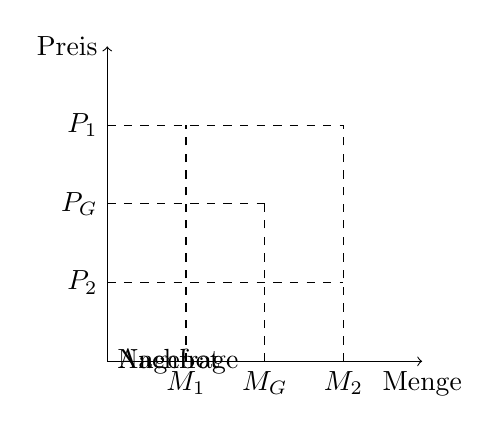
\begin{tikzpicture}
    %\draw[very thin,color=gray] (-0.1,-1.1) grid (3.9,3.9);
    \draw[->] (0,0) -- (4,0) node[below] {Menge};
    \draw[->] (0,0) -- (0,4) node[left] {Preis};
    \draw [thick, domain=0.1:3.6] plot[id=a] function{x} node [right] {Angebot};
    \draw [thick, domain=0.1:3.6] plot[id=n] function{-x + 4}  node [right] {Nachfrage};
	% Gleich
	\draw [dashed] (0,2) node [left] {$P_G$} -- (2, 2);
	\draw [dashed] (2,0) node [below] {$M_G$} -- (2, 2);
	% Angebot
	\draw [dashed] (0,3) node [left] {$P_1$} -- (3, 3);
	\draw [dashed] (3,0) node [below] {$M_2$} -- (3, 3);
	% Gleich
	\draw [dashed] (0,1) node [left] {$P_2$} -- (3, 1);
	\draw [dashed] (1,0) node [below] {$M_1$} -- (1, 3);	
\end{tikzpicture}
\end{center}

\begin{itemize}\itemsep0em
	\item Zum Preis $P_1$ wird die Menge $M_1$ nachgefragt, und die Menge $M_2$ angeboten.
	Die Angebot ist grösser als die Nachfrage $\Leftrightarrow$ Angebotsüberschuss.
	\item Zum Preis $P_2$ wird die Menge $M_2$ nachgefragt, und die Menge $M_1$ angeboten.
	Die Nachfrage ist grösser als das Angebot $\Leftrightarrow$ Nachfrageüberschuss.
	\item Am Punkt $(M_G, P_G)$ befindet sich der Markt im Gleichgewicht.
\end{itemize}

\subsection{Analyse von Marktveränderungen}
\begin{enumerate}\itemsep0em
	\item Entscheiden, ob ein Ereignis, die Nachfrage, die Angebots oder beide Kurven verschiebt
	\item Entscheiden, in welcher Richtung die Kurven verschoben werden
	\item Wirkung der Verschiebung im Diagramm hinsichtlich Gleichgewichtspreis und -menge untersuchen 
\end{enumerate}

\subsubsection{Verschiebungen}
\begin{itemize}\itemsep0em
	\item Nachfrage: rechts $\rightarrow$ Nachfrageüberschuss $\rightarrow$ Preis, Menge $\uparrow$
	\item Angebot nach links:
	\begin{itemize}
		\item elastisches Gut: Umstieg auf Substitute $\rightarrow$ Preis und Menge sinken (Anbieter tragen Steuerlast)
		\item unelatisches Gut: Preise steigen, Menge bleibt gleich (Nachfrager tragen Steuerlast)
	\end{itemize}
\end{itemize}

Für Preise ist vor allem der Grenznutzen entscheidend: Bei Wasser klein, bei Diamanten hoch.